\documentclass{article}

\usepackage{geometry}
\usepackage[utf8]{inputenc, vietnam}
\usepackage{graphicx}
\usepackage{amsmath, amssymb}

\geometry{a5paper}

\title{Phá mã vi sai (Differential Cryptanalysis)}
\author{Lê Quốc Dũng}

\newcommand{\PBox}{\text{PBox}}
\newcommand{\SBox}{\text{SBox}}
\newcommand{\Expand}{\text{Expand}}

\begin{document}

\maketitle

\section{TinyDES}

TinyDES là một phiên bản thu nhỏ của chuẩn mã hóa DES. TinyDES
là mã hóa khối theo mô hình Feistel, kích thước khối là 8 bit, kích
thước khóa cũng là 8 bit. Mỗi vòng khóa con có độ dài 6 bit.

\begin{figure}[ht]
    \centering
    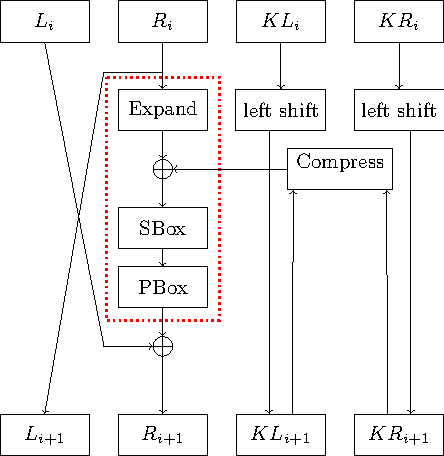
\includegraphics{../../pics/tinydes/blocky.pdf}
    \caption{Một vòng TinyDES}
\end{figure}

Mã TinyDES khá đơn giản. Theo mô hình Feistel, khối đầu vào 8 bit được chia thành
hai nửa trái phải 4 bit. Nửa phải sẽ đi qua các hàm Expand, SBox và PBox, sau đó
XOR với nửa trái để được nửa phải mới. Còn nửa trái mới là nửa phải cũ. Tóm lại 
công thức mô hình Feistel là
\[L_{i+1} = R_i, \quad R_{i+1} = L_i \oplus F(R_i, K_{i+1})\]
với $i = 1, 2, 3$ tương ứng 3 vòng với đầu vào của khối là $(L_0, R_0)$.

Chúng ta cần các động tác sau:

\begin{enumerate}
    \item Expand: mở rộng và hoán vị $R_i$ từ 4 bit lên 6 bit. Giả sử 4 bit
    của $R_i$ là $b_0 b_1 b_2 b_3$ thì kết quả sau khi Expand là $b_2 b_3 b_1
    b_2 b_1 b_0$;
    \item SBox: gọi 6 bit đầu vào là $b_0 b_1 b_2 b_3 b_4 b_5$. Khi đó ta tra
    cứu theo bảng SBox với $b_0 b_5$ chỉ số \textbf{hàng}, $b_1 b_2 b_3 b_4$ chỉ
    số \textbf{cột}. Nói cách khác bảng SBox có 4 hàng, 16 cột. Kết quả của SBox
    là một số 4 bit;
    \item PBox: là hàm hoán vị 4 bit $b_0 b_1 b_2 b_3$ thành $b_2 b_0 b_3 b_1$
\end{enumerate}

Như vậy, hàm $F$ của mô hình Feistel đối với mã TinyDES là
\[F(R_i, K_i) = PBox(SBox(Expand(R_i) \oplus K_{i+1}))\]

Để sinh khóa con cho 3 vòng, khóa ban đầu được chia
thành hai nửa trái phải lần lượt là $KL_0$ và $KR_0$. 
TinyDES thực hiện như sau:

\begin{enumerate}
    \item Vòng 1: $KL_0$ và $KR_0$ được dịch vòng trái 1 bit để được $KL_1$ và $KR_1$;
    \item Vòng 2: $KL_1$ và $KR_1$ được dịch vòng trái 2 bit để được $KL_2$ và $KR_2$;
    \item Vòng 3: $KL_2$ và $KR_2$ được dịch vòng trái 1 bit để được $KL_3$ và $KR_3$.
\end{enumerate}

Khi đó, khóa $K_i$ ở vòng thứ $i$ (với $i = 1, 2, 3$) là hoán vị và nén 8 bit
của $KL_i$ và $KR_i$ lại thành 6 bit. Đặt 8 bit khi ghép $KL_i \Vert KR_i$ là 
$k_0 k_1 k_2 k_3 k_4 k_5 k_6 k_7$, kết quả là 6 bit $k_5 k_1 k_3 k_2 k_7 k_0$.

\section{Phá mã vi sai (Differential Cryptanalysis)}

Giả sử $X_1$ và $X_2$ là hai khối input có cùng số bit.

Ta định nghĩa vi sai của $X_1$ và $X_2$ là $X = X_1 \oplus X_2$.

Xét các phép biến đổi trong TinyDES

\subsection{Phép XOR key}

Gọi $K$ là khóa con ở vòng nào đó trong thuật toán. Khi đó nếu đặt 
$Y_1 = X_1 \oplus K$ và $Y_2 = X_2 \oplus K$ thì vi sai của output là
$Y = Y_1 \oplus Y_2 = X_1 \oplus X_2$. Như vậy $K$ không tác động lên vi
sai và đây là tính chất quan trọng để chúng ta phá mã vi sai.

\subsection{Phép PBox}

Phép PBox bảo toàn số bit (hoán vị 4 bit thành 4 bit) và cách xây dựng hoán vị là
một biến đổi tuyến tính. Việc hoán vị 4 bit $b_0 b_1 b_2 b_3$ thành $b_2 b_0 b_3 b_1$
tương đương với phép nhân ma trận

\[
    \begin{pmatrix}
        0 & 0 & 1 & 0 \\
        1 & 0 & 0 & 0 \\
        0 & 0 & 0 & 1 \\
        0 & 1 & 0 & 0
    \end{pmatrix} \times
    \begin{pmatrix}
        b_0 \\ b_1 \\ b_2 \\ b_3
    \end{pmatrix} =
    \begin{pmatrix}
        b_2 \\ b_0 \\ b_3 \\ b_1
    \end{pmatrix}
\]

Do đó nếu đặt $Y_1 = \PBox (X_1)$ và $Y_2 = \PBox (X_2)$
thì \[Y_1 \oplus Y_2 = \PBox(X_1) \oplus \PBox(X_2) = \PBox(X_1 \oplus X_2)\]

Như vậy nếu vi sai input là cố định thì vi sai output cũng cố định do tính tuyến 
tính.

\subsection{Phép Expand}

Tương tự, phép Expand cũng là biến đổi tuyến tính và nếu đặt $Y_1 = \Expand(X_1)$
và $Y_2 = \Expand(X_2)$ thì \[Y_1 \oplus Y_2 = \Expand(X_1) \oplus \Expand(X_2)
= \Expand(X_1 \oplus X_2)\]

Cũng tương tự, nếu vi sai input là cố định thì vi sai output cũng cố định.

\subsection{Phép SBox}

Phép SBox là một biến đổi không tuyến tính với input 6 bit và output 4 bit.

Đặt $Y_1 = \SBox(X_1)$ và $Y_2 = \SBox(X_2)$.

Với mỗi $X = X_1 \oplus X_2$ cố định thì cứ một giá trị $X_1$ sẽ có duy nhất
một giá trị $X_2$ cho ra vi sai $X$. Tuy nhiên vi sai output $Y_1 \oplus Y_2$
phân bố không đều nhau.

Thực hiện bruteforce đơn giản trên SBox với vi sai input $X = X_1 \oplus X_2$ 
có 6 bit, ta tìm được sự phân bố vi sai output $Y = Y_1 \oplus Y_2$.

Chúng ta mong muốn rằng trên một hàng có càng ít phần tử càng tốt. 
Từ đó sự phân bố xác suất sẽ dễ kiểm soát hơn.

Sau khi xem bảng phân phối vi sai input và output ta có thể thấy được rằng

\begin{enumerate}
    \item Nếu vi sai input $X = 0$ thì chắc chắn vi sai output $Y = 0$
    \item Nếu vi sai input $X = 16$ thì có 9 vi sai output $Y$
    \item Nếu vi sai input $X = 52$ thì có 8 vi sai output $Y$
\end{enumerate}

Dựa trên nhận xét này, chúng ta sẽ tấn công trên các $X_1$, $X_2$ mà 
$X = X_1 \oplus X_2 \in \{ 16, 52 \}$.

Xét hai hàng 16 và 52, ta thấy rằng

\begin{enumerate}
    \item Nếu vi sai input $X = 16$ thì vi sai output $Y = 7$ là cao nhất với
    xác suất $14/64$
    \item Nếu vi sai input $X = 52$ thì vi sai output $Y = 2$ là cao nhất với
    xác suất $16/64$
\end{enumerate}

\subsection{Hàm $F$}

Như vậy, phép XOR key, phép PBox và phép Expand cho xác suất đều nhau với các
cặp vi sai $(X, Y)$. Trong khi đó thì SBox lại cho xác suất các cặp vi sai $(X, Y)$
không đều nhau. 

Đặt $Y_1 = F(X_1)$ và $Y_2 = F(X_2)$. Dễ thấy rằng

\begin{itemize}
    \item Vi sai input của hàm $F$ chính là vi sai input của Expand
    \item Vi sai output của Expand là vi sai input của SBox (không phụ thuộc vào khóa)
    \item Vi sai output của SBox là vi sai input của PBox
    \item Vi sai output của PBox là vi sai output của hàm $F$
\end{itemize}

Ta có thể đưa ra nhận xét về xác suất 
vi sai output $Y = Y_1 \oplus Y_2$ từ vi sai $X = X_1 \oplus X_2$ như sau

\begin{enumerate}
    \item Nếu vi sai input của $F$ là 0 $\rightarrow$ vi sai output của Expand là 0
    $\rightarrow$ vi sai output của SBox chắc chắn là 0 $\rightarrow$ vi sai output
    của PBox chắc chắn là 0 $\rightarrow$ vi sai output của hàm $F$ chắc chắn là 0
    \item Nếu vi sai input của $F$ là 1 $\rightarrow$ vi sai output của Expand là 16
    $\rightarrow$ vi sai output của SBox là 7 với xác suất $14/64$ $\rightarrow$ vi
    sai output của PBox là 11 với xác suất là $14/64$ $\rightarrow$ hàm $F$ là 11 
    với xác suất $14/64=7/32$
    \item Nếu vi sai input của $F$ là 3 $\rightarrow$ vi sai output của SBox là 52
    $\rightarrow$ vi sai output của SBox là 2 với xác suất $16/64$ $\rightarrow$ vi
    sai output của PBox là 8 với xác suất $16/64$ $\rightarrow$ hàm $F$ là 8
    với xác suất $16/64 = 1/4$
\end{enumerate}

\subsection{Chosen plaintext part 1}

Do tính chất vi sai, chúng ta sẽ mong muốn tìm những cặp (plaintext, ciphertext) $(P_1, C_1)$
và $(P_2, C_2)$ nào đó mà vi sai input $P_1 \oplus P_2$ và vi sai output $C_1 \oplus C_2$
có thể tối ưu xác suất trên.

Giả sử chúng ta xét trường hợp 3 ở trên, khi vi sai input của $F$ là 3 thì vi sai output
của $F$ là 8 với xác suất $1/4$. Đây là xác suất lớn nhất nên ta mong muốn trong 3 vòng
của TinyDES sẽ tận dụng được càng nhiều càng tốt.

Chúng ta đi từ dưới lên. Đặt
\[L_3 = R_2, \quad R_3 = L_2 \oplus F(R_2, K_3)\]
và
\[L_3' = R_2', \quad R_3' = L_2' \oplus F(R_2', K_3)\]

Chọn $R_2 \oplus R_2' = 3$ thì $F(R_2, K_3) \oplus F(R_2', K_3) = 8$ với
xác suất $1/4$. Vì là bước cuối nên ta hy vọng ciphertext cuối cùng sẽ càng ít phức
tạp càng tốt. Do đó có thể lựa chọn $L_2 = L_2' = 0$ để bảo toàn vi sai sau khi vòng 
3 kết thúc.

\textbf{Ở vòng 3, xác suất để vi sai input bằng 3 và vi sai output bằng 8 là $1/4$}.

Tiếp theo, đặt
\[L_2 = R_1, \quad R_2 = L_1 \oplus F(R_1, K_2)\]
và
\[L_2' = R_1', \quad R_2' = L_1' \oplus F(R_1', K_2)\]

Do $L_2 = R_1$ nên $R_1 = 0$. Tương tự $R_1' = L_2' = 0$. Điều đáng chú ý là 
$R_1 \oplus R_1' = 0$, nghĩa là vi sai input bằng 0, nên vi sai output 
$F(R_1, K_2) \oplus F(R_1', K_2)$ chắc chắn bằng 0 (xác suất bằng 1).

\textbf{Ở vòng 2, xác suất để vi sai input bằng 0 và vi sai output bằng 0 là 1}.

Ta lại có 
\[R_2 \oplus R_2' = 3 = L_1 \oplus F(R_1, K_2) \oplus L_1' \oplus 
F(R_1', K_2) = L_1 \oplus L_1'\]
do vi sai output hàm $F$ chắc chắn bằng 0. Do đó $L_1 \oplus L_1' = 3$.

Tuy nhiên, $L_1 = R_0$ và $L_1' = R_0'$ nên $L_1 \oplus L_1' = R_0 \oplus R_0' = 3$.
Do đó vi sai output của hàm $F$ là $F(R_0, K_1) \oplus F(R_0', K_1) = 8$ có xác suất
$1/4$. 

\textbf{Ở vòng 1, xác suất để vi sai input bằng 3 và vi sai output bằng 8 là $1/4$}.

Cuối cùng 
\[R_1 \oplus R_1' = L_0 \oplus F(R_0, K_1) \oplus L_0' \oplus F(R_0', K_1) =
L_0 \oplus L_0' \oplus 8\]
mà ta nhớ lại ở trên $R_1 \oplus R_1' = 0$ nên suy ra $L_0 \oplus L_0' = 8$.

Tổng kết lại, ta chọn vi sai input $(L, R) = (8, 3)$ thì xác suất để vi sai output
bằng $(3, 8)$ là $(1/4) \times 1 \times (1/4) = 1/16$. Đây là xác suất cao nhất
có thể sau khi TinyDES chạy đủ 3 vòng.

\subsection{Chosen plaintext part 2}

Tương tự, chúng ta xét trường hợp 2 ở trên, khi vi sai input của $F$ là 1 thì vi sai 
output của $F$ là 11 với xác suất $7/32$. Ta cũng mong muốn sau 3 vòng của TinyDES
sẽ tận dụng được càng nhiều càng tốt.

Chúng ta lại đi dưới lên. Đặt
\[L_3 = R_2, \quad R_3 = L_2 \oplus F(R_2, K_3)\]
và
\[L_3' = R_2', \quad R_3' = L_2' \oplus F(R_2', K_3)\]

Chọn $R_2 \oplus R_2' = 1$ thì $F(R_2, K_3) \oplus F(R_2', K_3) = 11$ với xác suất
$7/32$. Vì là bước cuối cùng nên ta cũng hy vọng ciphertext sẽ càng ít phức tạp càng
tốt. Do đó ta chọn $L_2 = L_2' = 0$.

\textbf{Ở vòng 3, xác suất để vi sai input bằng 1 và vi sai output bằng 11 là 7/32}.

Tiếp theo, đặt
\[L_2 = R_1, \quad R_2 = L_1 \oplus F(R_1, K_2)\]
và
\[L_2' = R_1', \quad R_2' = L_1' \oplus F(R_1', K_2)\]

Do $L_2 = R_1$ nên $R_1 = 0$. Tương tự $R_1' = 0$. Suy ra $R_1 \oplus R_1' = 0$
và vi sai output $F(R_1, K_2) \oplus F(R_1', K_2) = 0$ với xác suất bằng 1 (chắc
chắn xảy ra).

\textbf{Ở vòng 2, xác suất để vi sai input bằng 0 và vi sai output bằng 0 là 1}.

Ta lại có

\[R_2 \oplus R_2' = L_1 \oplus F(R_1, K_2) \oplus L_1' \oplus F(R_1', K_2) = L_1 \oplus L_1'\]
do vi sai output của hàm $F$ chắc chắn bằng 0. Do đó $L_1 \oplus L_1' = 1$.

Tuy nhiên $L_1 = R_0$ và $L_1' = R_0'$ nên $R_0 \oplus R_0' = L_1 \oplus L_1' = 1$.
Do đó vi sai output của hàm $F$ ở vòng 1 là $F(R_0, K_1) \oplus F(R_0', K_1) = 11$ với
xác suất $7/32$.

\textbf{Ở vòng 1, xác suất để vi sai input bằng 1 và vi sai output bằng 11 là 7/32}.

Cuối cùng, do 
\[R_1 \oplus R_1' = L_0 \oplus F(R_0, K_1 \oplus L_0' \oplus F(R_0', K_1))\]
mà $R_1 \oplus R_1' = 0$ và $F(R_0, K_1) \oplus F(R_0', K_1) = 11$ nên 
$L_0 \oplus L_0' = 11$.

Tổng kết lại, ta chọn vi sai input $(L, R) = (11, 1)$ thì xác suất để vi sai output
bằng $(1, 11)$ là $(7/32) \times 1 \times (7/32) \approx 0.048$. Đây cũng là xác suất
cao nhất có thể sau khi TinyDES chạy đủ 3 vòng.

\subsection{Final attack}

Như vậy, đối với TinyDES chúng ta phá mã vi sai như sau

\begin{enumerate}
    \item Tìm một số lượng cặp plaintext, ciphertext $(P_1, C_1)$, $(P_2, C_2)$, ...
    cho tới khi tìm được $P_i \oplus P_j = 0x83$ và $C_i \oplus C_j = 0x38$
    \item Tìm một số lượng cặp plaintext, ciphertext $(P_1', C_1')$, $(P_2', C_2')$, ...
    cho tới khi tìm được $P_i' \oplus P_j' = 0xB1$ và $C_i' \oplus C_j' = 0x1B$
\end{enumerate}

Sau khi đã tìm được một số lượng cặp plaintext, ciphertext thỏa vi sai trên, nhớ
lại hàm $F$ ở vòng 3, do $L_3 = R_2$ và $R_3 = L_2 \oplus F(R_2, K_3) = 
L_2 \oplus F(L_3, K_3) = F(L_3, K_3)$ (ta chọn $L_2 = 0$ ở trên), dễ thấy rằng
chúng ta có thể tìm được các $K_3$ thỏa mãn hàm $F$ ở vòng 3.

Để làm điều đó thì ta tính $O = \Expand(L_3)$, và do $\SBox(O \oplus K_3) =
\PBox^{-1}(R_3)$ cũng tính được nên có thể tìm các giá trị $O \oplus K_3$ mà khi đi
qua $\SBox$ cho kết quả bằng $\PBox^{-1}(R_3)$. Sau đó XOR lại cho $O$ thì sẽ tìm
được các giá trị có thể của $K_3$. Lưu ý rằng $\SBox$ làm giảm 6 bit còn 4 bit nên
sẽ có nhiều giá trị khác nhau cho cùng giá trị $\SBox$.

Thực hiện trên hai trường hợp vi sai input-output là $(0x83, 0x38)$ và $(0xB1, 0x1B)$
ta có tập các giá trị có thể xảy ra của $K_3$.

Theo thuật toán sinh khóa con thì với khóa $K$ 8 bit ban đầu, đặt là $k_0 k_1 k_2 k_3
k_4 k_5 k_6 k_7$, thì khóa con $K_3$ là $k_5 k_1 k_3 k_2 k_7 k_0$. Trong $K_3$ không
có $k_4$ và $k_6$ nên chúng ta sẽ bruteforce hai bit này tới khi tìm được đúng khóa
$K$ mà tương ứng với cặp $(P_i, C_i)$.
\end{document}